\subsubsection{DFUSe Programm}
\label{sec:DFUSe}

STMicroelectronics stellt eine Software namens DfuSe zur Verfügung um die Firmware STM32 Devices ohne Debugger zu programmieren.
\todo{SB - cite auf Download link}

\paragraph{HEX File zu DFU File konvertieren}

Für den Prozess verlangt das Tool, ein \texttt{.dfu} Dateiformat, dass nicht von der IDE erzeugt wird. 
Im Normalfall ist die kompilierte Binärdatei aus Keil uVision 5 im \texttt{.hex} Format im Projektordner unter \texttt{./MDK-ARM/<Projektname>/<Projektname>.hex} zu finden.\\

Das DfuSe Tool kommt mit einem weiteren Werkzeug, um Dateien vom \texttt{.hex} ins \texttt{.dfu} Format zu konvertieren. 
Dieses heisst DFU File Manager und ist in Abbildung \ref{pic:DFU_file_man} dargestellt.

\begin{figure}[H]
	\centering
	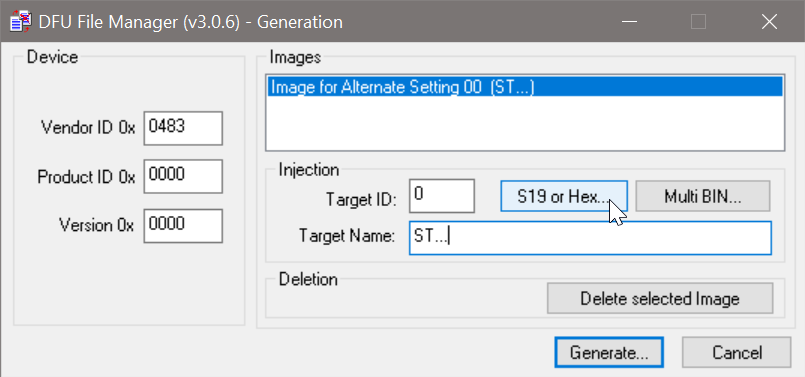
\includegraphics[width=0.5\linewidth]{DFU_file_man}
	\caption{Firmware Upgrade Tool DfuSe}
	\label{pic:DFU_file_man}
\end{figure}

Den DFU File Manager starten und \textit{"I want to GENERATE a DFU file from HEX"} auswählen.
Darauf präsentiert sich das Tool wie in Abbildung \ref{pic:DFU_file_man}. Hier kann eine \texttt{.hex} Datei ausgewählt und anschliessend konvertiert und gespeichert werden.
Mit Klick auf \textit{"S19 or HEX..."} kann das \texttt{<Projektname>.hex} ausgewählt und anschliessend mit Klick auf \textit{"Generate..."} ein \texttt{<Projektname>.dfu} generiert werden.

\paragraph{DFU Datei auf das DSP Board programmieren}

Die nun erstellte \texttt{<Projektname>.dfu} Datei kann mit dem DfuSe Programm auf das im DFU Modus gebootete DSP-Board programmiert werden. 
Die Abbidung \ref{pic:DFUSe_Upgrade} zeigt das DfuSe Programm, bei dem das DSP-Board bereits am USB Port erkannt wurde. Die Erkennung geschieht automatisch, sofern das DSP-Board über USB am Computer angeschlossen ist und sich im Bootloader befindet.

\begin{figure}[H]
	\centering
	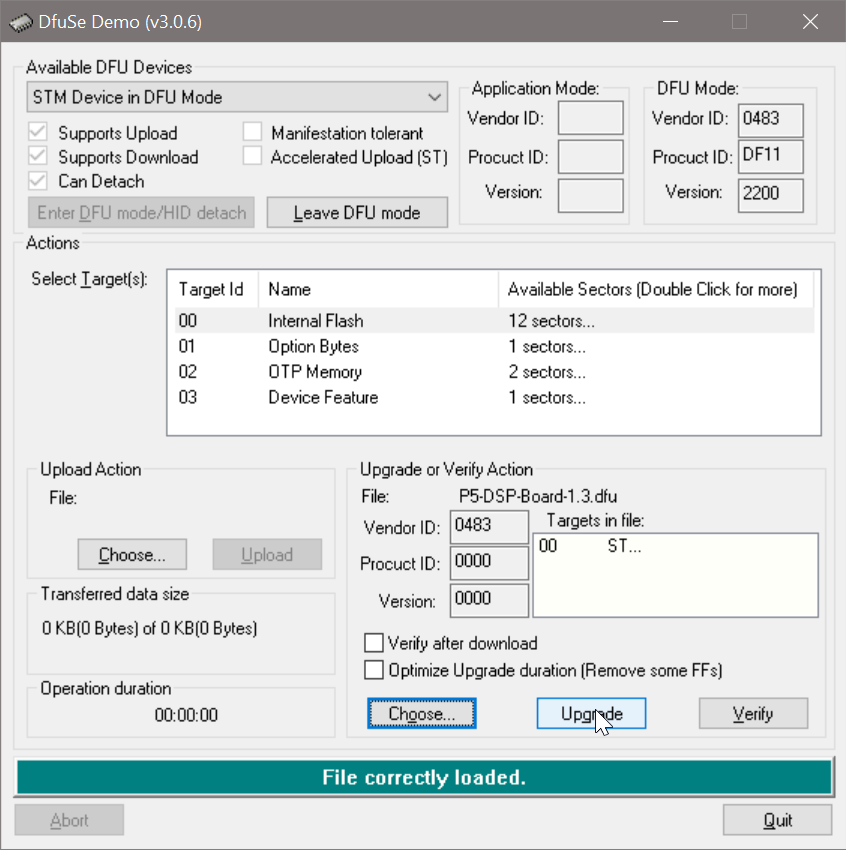
\includegraphics[width=0.65\linewidth]{DFUSe_Upgrade}
	\caption{Firmware Upgrade Tool DfuSe}
	\label{pic:DFUSe_Upgrade}
\end{figure}

Mit Klick auf \textit{"Choose..."} wird die \texttt{<Projektname>.dfu} ausgewählt.
Anschliessend mit \textit{"Upgrade"} die neue Firmware programmieren.
Dabei erscheint eine Warnung \textit{"...it is impossible to make sure this file is for device."}, welche mit \textit{"Yes"} bestätigt werden kann.

Wenn das Upgrade vollzogen ist, erscheint der Balken unten in grün. Jetzt kann das DSP-Board mit \textit{"Leave DFU Mode"} neu gestartet werden.


